\section{Formalization}\label{sec:formal}

% \begin{itemize}
% \item Describe the types for checked-C as a graph. \dvh{I don't know what this means.}

% \item Describe the subtyping for checked-C types.
% \begin{itemize}
% \item State that the subtypes in Checked-C are transitive.
% \end{itemize}

% \item Describe the syntax of Checked-C

% \item Describe the semantics of Checked-C

% \item Describe the type system of Checked-C

% \item Describe the progress and preservation theorems, and outline the proofs.

% \item Describe the blame theorem and proof.

% \end{itemize}

% \ignore{
% \begin{figure}
%   \begin{center}
%     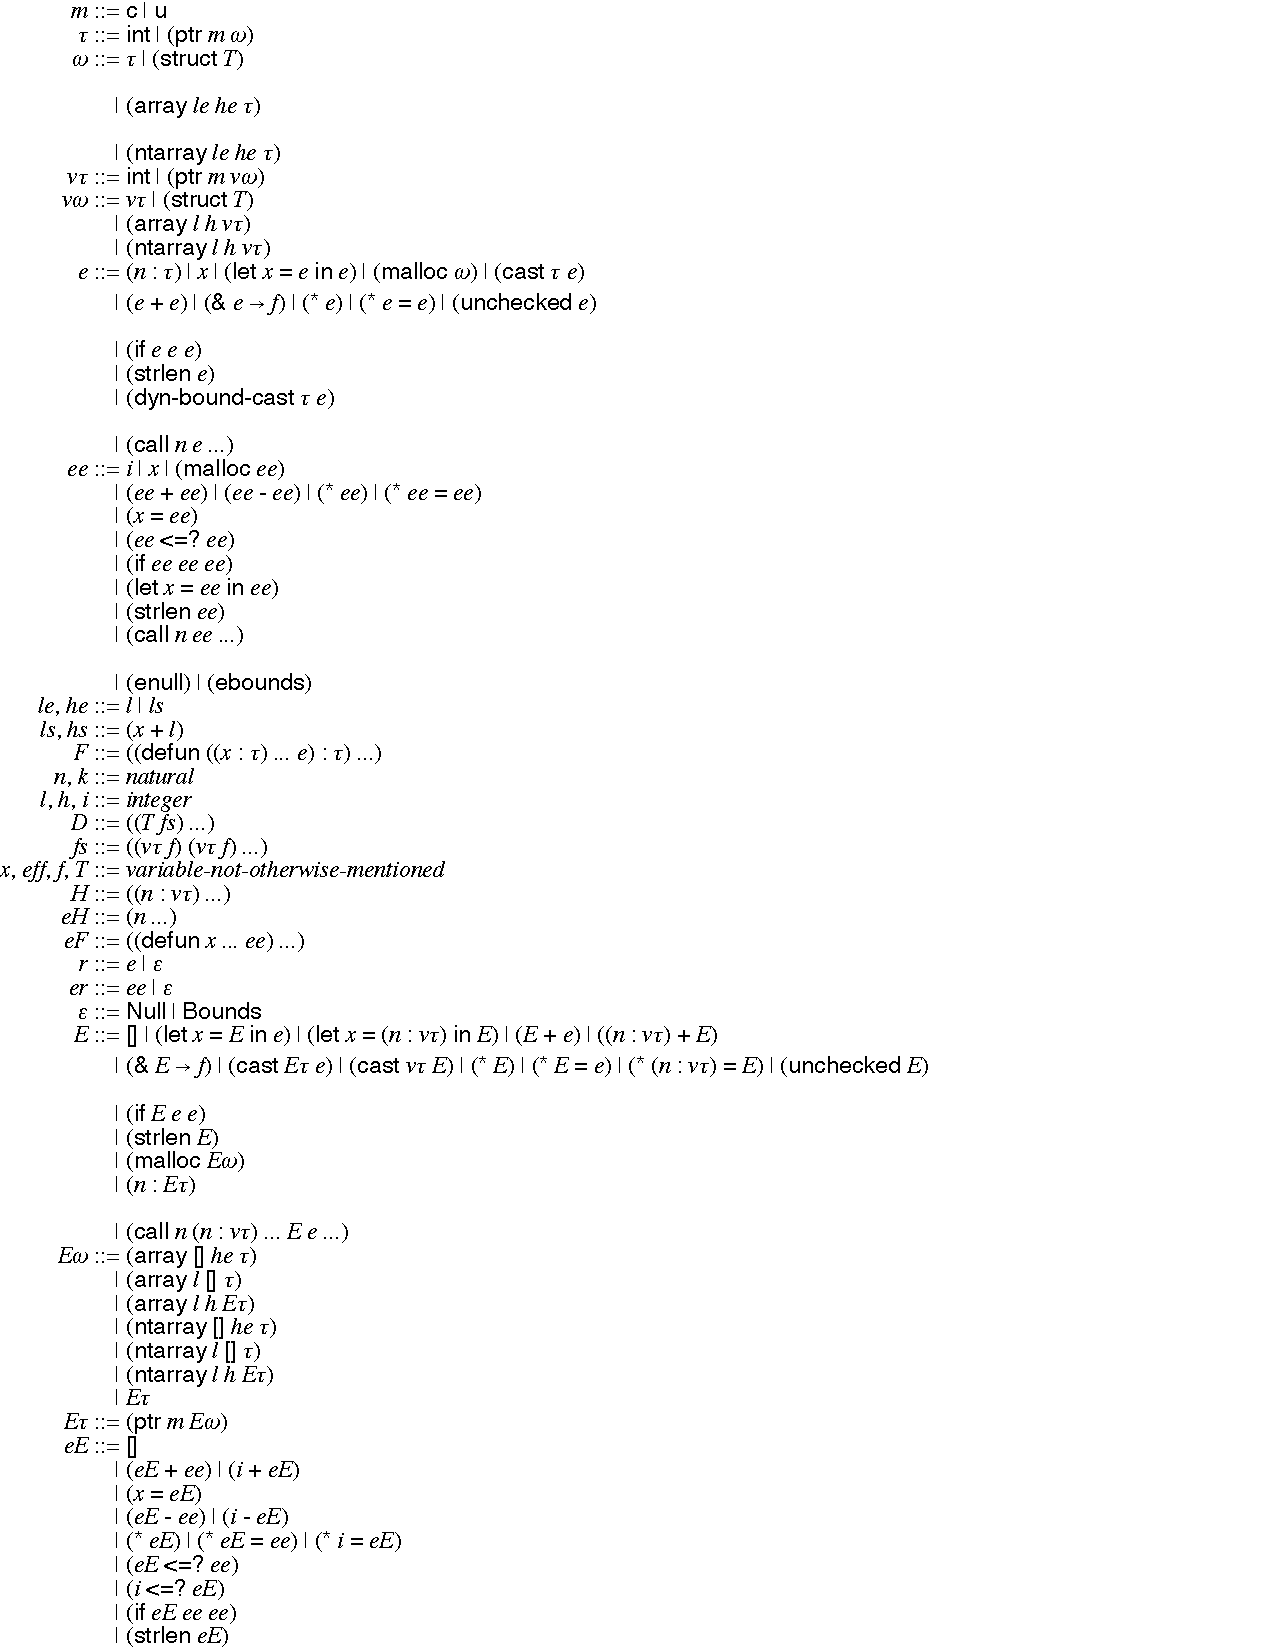
\includegraphics[height=6in]{syntax.pdf}
%   \end{center}
%   \caption{\lang: Syntax}
% \end{figure}

% \begin{figure}
%   \begin{center}
%     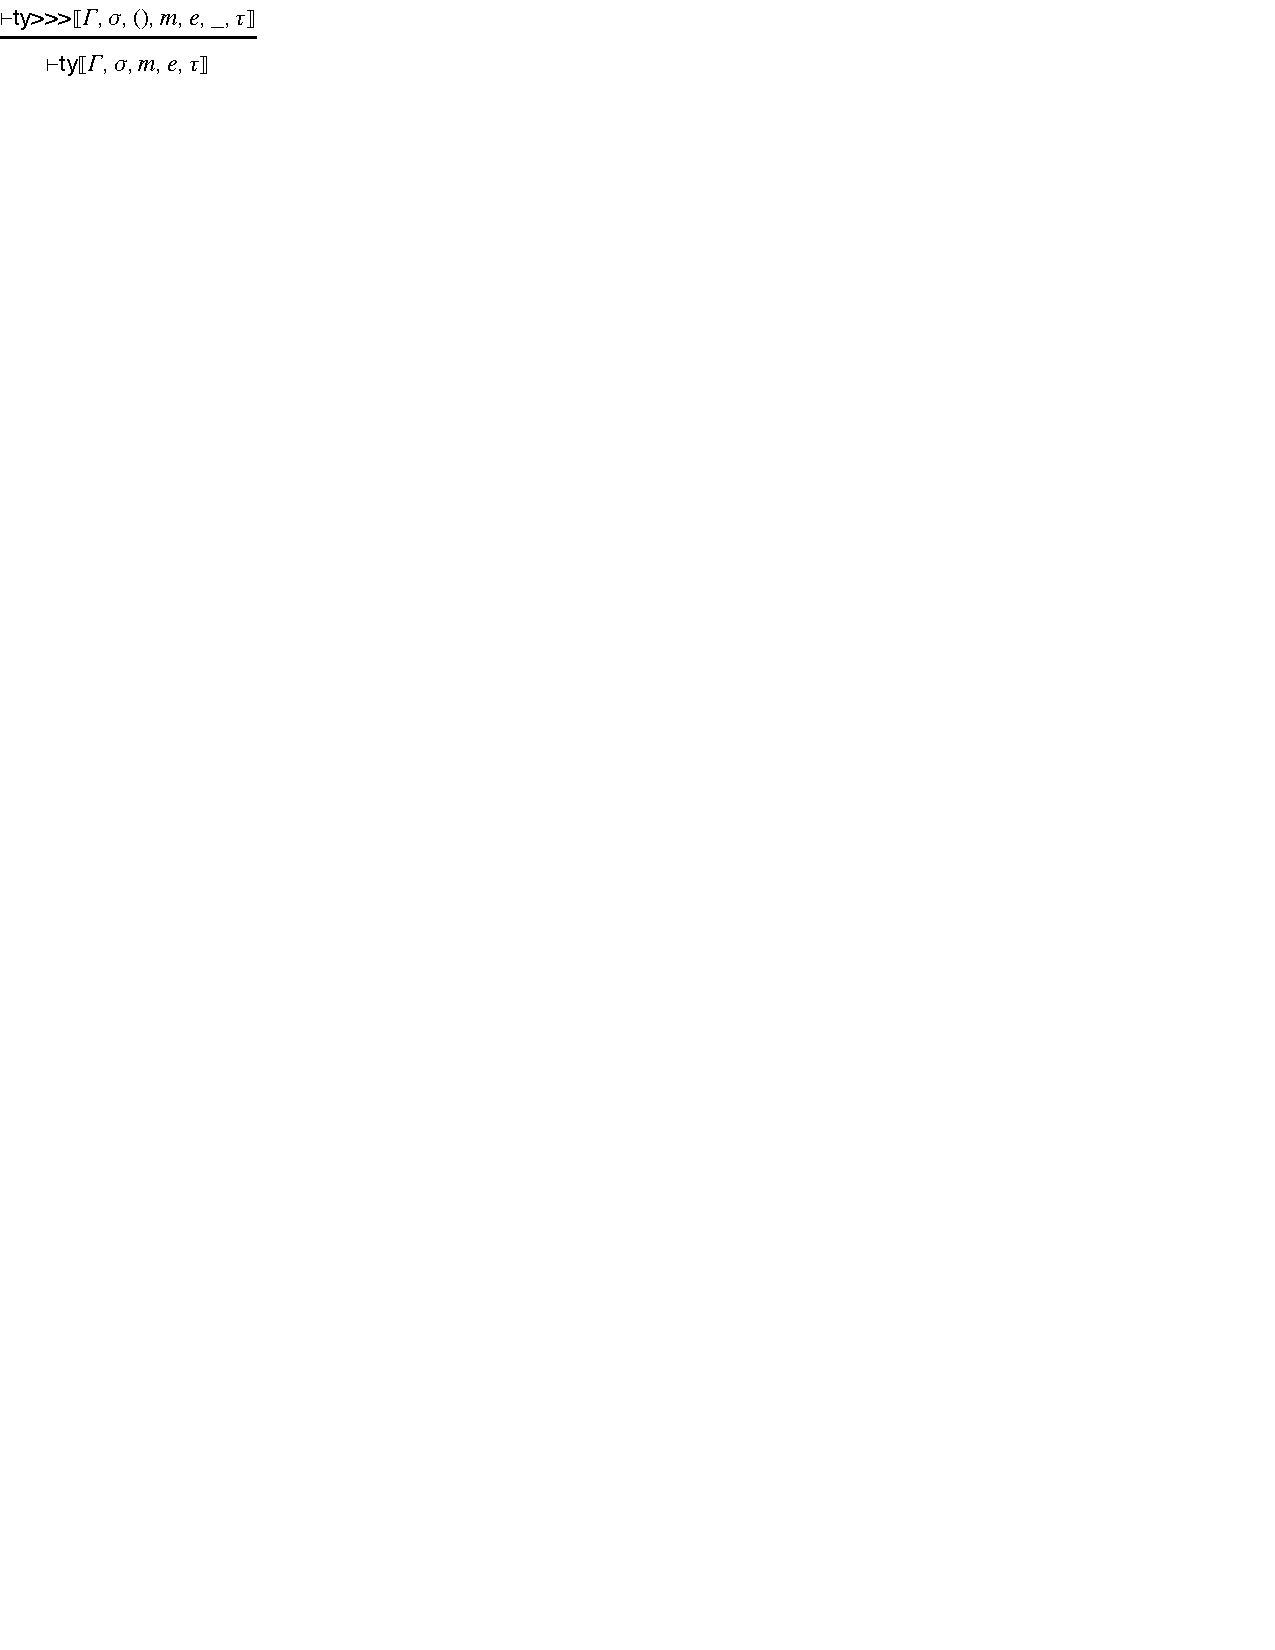
\includegraphics[height=6in]{types.pdf}
%   \end{center}
%   \caption{\lang: Typing}
% \end{figure}
% }
% \liyi{main text begins here. }

% \review{
% While reading the semantics, I found the fact that S-Def and S-DefNull are
%   applicable non-deterministically if n is 0 a bit confusing. Only when
%   reading the meta-theory section I realized that this is not a concrete issue
%   because well-formed heaps are such that $\mathcal{H}(0)$ is never defined. It
%   might be worth pointing this out early on. }
% \mwh{Done.}

\begin{figure}
  \small \centering
  $\begin{array}{l}
\begin{array}{lll}
\text{Function names:}~f&
       \text{Variables:}~ x
& \text{Integers:}~n::=\mathbb{Z} 
\end{array}
\\[0.5em]

\begin{array}{llcllcl}

\text{Mode:} & m & ::= & \cmode \mid \umode \\[0.5em]

\text{Bound:} & b & ::= & n \mid x \plus n \\
              & \bvar & ::= & (b,b) \\[0.5em]
  
     \text{Word Type:}& \tau &::=& \tint\mid \tptr{\omega}{m}
\\[0.5em]

\text{Type Flag:}&\kappa &::=& nt \mid \cdot
\\[0.5em]

\text{Type:}&\omega &::=& \tau \mid \tallarrayb{\bvar}{\tau}
\\[0.5em]

\text{Expression:}& e & ::= & 
\evalue{n}{\tau} \mid x \mid \emalloc{\omega} \mid\elet{x}{e}{e} \\[0.2em]
&&\mid&
\ecast{\tau}{e} \mid \edyncast{\tau}{e}\mid \ecall{f}{\overline{e}} \mid \estrlen{x} \\[0.2em]
&&\mid&
\ebinop{e}{e} \mid\estar{e}\mid\eassign{e}{e}\mid\eunchecked{e}
\\[0.2em]
&&\mid&\eif{e}{e}{e}
\end{array}
    \end{array}
  $
  \caption{\lang Syntax}
  \label{fig:checkc-syn}
\end{figure}

%% \dvh{I don't understand the variable grammar.  What is $T$?  What is $\eta$?  I think $\cmode$ and $\umode$ should be in tt font.}
%% \liyi{T and $\eta$ can be moved to the appendix, they are useful only for struct types.}

% \review{
% - Furthermore, inspecting the code also suggests that the expression type (line 155) does not contain constructors for function calls (and I don't see a way to define functions either), conditionals, or strlen, and doesn't distinguish between the two forms of casting. All this contradicts figure 2, and should be clarified
% }
% \liyi{It is in the CheckedC.v file, 392. }
% \mwh{How is this answer helping the reviewer since you've added
%   nothing to the text? Maybe we should add something to an appendix
%   that matches the formalism shown in the paper to definitions in the
%   Coq file?}
% \liyi{The detailed explanation is in the appendix.}

This section describes our formal model of \checkedc, called
\lang, making precise its syntax, semantics, and type system. It also
develops \lang's meta-theory, including type soundness and the blame
theorem.

\subsection{Syntax}\label{sec:syntax}

The syntax of \lang is given by the expression-based
language presented in Fig.~\ref{fig:checkc-syn}.

There are two notions of type in \lang.  Types $\tau$ classify
word-sized values including integers and pointers, while types
$\omega$ classify multi-word values such as arrays, null-terminated
arrays, and single-word-size values.
%
Pointer types ($\tptr{\omega}{m}$) include a mode annotation ($m$)
which is either checked (\cmode) or unchecked (\umode) and a type
($\omega$) denoting valid values that can be pointed to. Array types include both the type of
elements ($\tau$) and a bound ($\bvar$) comprised of an upper and
lower bound on the size of the array ($(b_l,b_h)$). Bounds $b$ are
limited to integer literals $n$ and expressions $x + n$.
Whether an array pointer is null terminated or not is determined by annotation
$\kappa$, which is $nt$ for null-terminated arrays, and $\cdot$
otherwise (we elide the $\cdot$ when writing the type). Here is the
corresponding \checkedc syntax for these types:
\[
\begin{array}{rcl}
$\code{array_ptr<}$\tau$\code{> : count(}$n$\code{)}$
&\Leftrightarrow& \tarrayptr{0}{n}{\tau}{\cmode}
\\[0.2em]
$\code{nt_array_ptr<}$\tau$\code{> : count(}$n$\code{)}$
&\Leftrightarrow& \tntarrayptr{0}{n}{\tau}{\cmode}
\end{array}
\]
As a convention we write $\tptr{\tarrayb{b}{\tau}}{\cmode}$ to mean
$\tptr{\tarray{0}{b}{\tau}}{\cmode}$, so the above examples could
be rewritten $\tptr{\tarrayb{n}{\tau}}{\cmode}$ and
$\tptr{\tntarrayb{n}{\tau}}{\cmode}$, respectively.

\lang expressions include literals ($n\!:\!\tau$), variables ($x$), memory
allocation ($\emalloc{\omega}$), let binding ($\elet{x}{e_1}{e_2}$),
static casts ($\ecast{\tau}{e}$), dynamic casts ($\edyncast{\tau}{e}$)
(assumed at compile-time and verified at run-time, see Sec.~\ref{sec:example}),
function calls ($\ecall{f}{\overline{e}}$), addition
($\ebinop{e_1}{e_2}$), pointer dereference and assignment ($\estar{e}$)
and ($\eassign{e_1}{e_2}$), resp.), unchecked blocks ($\eunchecked{e}$),
the \texttt{strlen} operation ($\estrlen{x}$), and conditionals ($\eif{e}{e_1}{e_2}$).
% \review{III.A.: the "dynamic cast" terminology may be briefly confused for C++'s
%   RTTI-based dynamic cast feature}
% \mwh{Added reference back to Section 2-B}

Integer literals $n$ are annotated with a type $\tau$ which can be either
$\tint$, or $\tptr{\omega}{m}$ in the case $n$ is being used as
a heap address (this is useful for the semantics);
$\evalue{0}{\tptr{\omega}{m}}$ (for any $m$ and $\omega$) represents
the $\enull$ pointer, as usual. 
The
$\texttt{strlen}$ expression operates on variables $x$
rather than arbitrary expressions to simplify managing
bounds information in the type system; the more general case can be
encoded with a \code{let}. We use a less verbose syntax for dynamic bounds
casts; e.g., the following %

\code{dyn_bounds_cast<array_ptr<}$\tau$\code{>>(}$e$\code{, count(}$n$\code{))}

\noindent
becomes $\edyncast{\tptr{\tarrayb{n}{\tau}}{\cmode}}{e}$. 

\lang aims to be simple enough to work with, but powerful enough to
encode realistic \checkedc idioms. For example, mutable local
variables can be encoded as immutable locals that point to the heap;
the use of \code{&} can be simulated with \code{malloc};
and loops can be encoded as recursive function calls. \code{struct}s are
not in Fig.~\ref{fig:checkc-syn} for space reasons, but they are
actually in our model, and developed in
\iftr
Appendix~\ref{appx:struct}.
\else
the supplemental report~\cite{checkedc-tech-report}.
\fi
C-style \code{union}s have no safe typing
in \checkedc, so we omit them. By default, functions are assumed to
be within checked regions; placing the body in an \code{unchecked}
expression relaxes this, and within that, checked regions can be
nested via function calls. Bounds are restricted slightly:
rather than allowing arbitrary sub-expressions, bounds must be either
integer literals or variables plus an integer offset, which accounts
for most uses of \code{bounds} in \checkedc programs. \lang bounds are
defined as relative offsets, not absolute ones, as in the second part
of Fig.~\ref{fig:checkedc-example}. We see no technical problem to
modeling absolute bounds, but it would be a pervasive change so we
have not done so.

  We have mechanized two models of \lang, one in Coq
  and one in PLT Redex~\cite{pltredex}, which is a semantic
  engineering framework implemented in Racket. Redex provides direct
  support for specifying the operational semantics and typing with logical
  rules, but then automatically makes them executable and subject to
  randomized testing, which is very useful during development.
  The model we present in the paper faithfully
  represents both mechanizations, but there are some differences for
  presentation purposes. For example, the paper and the Coq model use an explicit
  stack, whereas the Redex model uses \code{let} bindings to simulate
  one (simplifying term generation for randomized
  testing).
\iftr
  Appendix~\ref{app:model-diffs} 
\else
  The supplemental report~\cite{checkedc-tech-report}
\fi
  outlines the differences
  between the two models and the paper formalism.

% \mwh{NOTE: COULD WORK THE FOLLOWING INTO THE ABOVE DESCRIPTION OF
%   POINTERS: Array and NT-array types have two relative bounds, whose structures
% can be either an integer or a variable plus an integer. For example,
% if we have the expression
% $x\texttt{=}\emalloc{\tarrayb{(0,10)}{\tint}}$, $x$ then has the type
% $\tptr{\tarrayb{10}{\tint}}{\cmode}$, which represents an array
% pointer of size $10$. The bounds ($(b_l,b_h)$ in
% $\evalue{p}{\tptr{\tarrayb{(b_l,b_h)}{\tau}}{m}}$) indicate relative
% offsets from this pointer of the accessible memory, i.e., $p+b_l$ and
% $p+b_h$. As such, a pointer can only be directly dereferenced if 0 is
% included within the annotated range.  If following the $\emalloctext$
% operation, we execute $*(x-1)$ and $*(x\plus 10)$. The two expressions
% are not valid, because the type of the two expressions $(x-1)$ and
% $(x\plus 10)$ are $\tarrayptr{1}{11}{\tint}{\cmode}$ and
% $\tarrayptr{-10}{0}{\tint}{\cmode}$ and $0$ in these two cases are not
% in the ranges: $[1,11)$ and $[-10,0)$. Thus, in order for a $\cmode$
% pointer with type $\tarrayptr{b_l}{b_h}{\tint}{\cmode}$ to be
% accessible in \checkedc, $0$ must be in the range of $[b_l,b_h)$.}

\begin{figure}
{\small
$    \begin{array}{l}
    \begin{array}{lll}
\mu & ::= & \evalue{n}{\tau} \mid \bot\\
e & ::= & \ldots \mid \ret{x}{\mu}{e}\\
r & ::= & e \mid \enull \mid \ebounds\\
E &::=& \Box \mid \elet{x}{E}{e} \mid \ecall{f}{\overline{E}}\mid\ecast{\tau}{E} \mid \edyncast{\tau}{E} \\[0.2em]
&& \mid \ebinop{\evalue{n}{\tau}}{E}\mid\estar{E}\mid\eassign{E}{e} \\[0.2em]
&&\mid\eassign{\evalue{n}{\tau}}{E}\mid\eunchecked{E}\mid\eif{E}{e}{e}\\[0.2em]
\overline{E} &::=& E \mid  \evalue{n}{\tau},\overline{E} \mid \overline{E}, e
\end{array}
\\ \\
    \end{array} 
$
  \begin{mathpar}
    \inferrule{ m=\mode(E) \\
      e=E[e'] \\
      (\varphi,\heap,e') \longrightarrow (\varphi',\heap',e'')}
    {(\varphi,\heap,e)\longrightarrow_{m} (\varphi',\heap',E[e''])}
 

    \inferrule{ m=\mode(E) \\
      e=E[\eif{\estar{x}}{e_1}{e_2}] \\
      (\varphi,\heap,\eif{\estar{x}}{e_1}{e_2})
              \longrightarrow (\varphi',\heap',e')}
    {(\varphi,\heap,e)\longrightarrow_{m} (\varphi',\heap',E[e'])}
    \;\;\;{[\emph{prefer}]}

  \end{mathpar}
}
  \caption{\lang Semantics: Evaluation}
  \label{fig:c-context}
\end{figure}

\subsection{Semantics}\label{sec:semantics}

% The semantics
% gives an independent account of spatial safety in \lang by
% checking pointer bounds based on the annotations carried on types at
% run-time.  While this account makes clear that bounds checking occurs
% as expected, it suggests an implementation that uses fat pointers to
% carry bounds.  We resolve this tension in the subsequent section on
% compilation and show that an implementation faithful to the semantics
% can be obtained without fat pointers.  
% \review{repeat that the stack is immutable at this point?}
% \liyi{Is it? Is the stack immutable? What does the immutable mean? 
%   In a stack, the variable values can be changed? Right?
%   The pointer address itself cannot be changed once it is created, but the stack variable content can be updated?  }
% \mwh{It certainly seems to be immutable: Your create stack frames
%   using let binding, and the let-bound variables will always be bound
%   to the same things. I.e., stack cells are immutable.}

% \review{this raises a fair amount of questions regarding the treatment of the
%   NULL pointer at this stage of the paper... is it modeled as 0, as returned by
%   `malloc`? are dynamic checks inserted by CheckedC to guarantee that no NULL
%   pointer is dereferenced?}
% \mwh{Yes, it is modeled as 0, and the semantics checks for
%   dereferences of 0. }

The operational semantics for \lang is defined as a small-step
transition relation with the judgment $ (\varphi,\heap,e)
\longrightarrow_m (\varphi',\heap',r)$. Here, $\varphi$ is a
\emph{stack} mapping from variables to values $\evalue{n}{\tau}$ and
$\heap$ is a \emph{heap} mapping addresses (integer literals) to
values $\evalue{n}{\tau}$; for both we ensure
$\fv(\tau)=\emptyset$.
While heap bindings can change, stack bindings are immutable---once
variable $x$ is bound to $\evalue{n}{\tau}$ in $\varphi$, that binding will not
be updated; we can model mutable stack variables as pointers into the
mutable heap.
As mentioned, value $\evalue{0}{\tau}$
represents a $\enull$ pointer when $\tau$ is a pointer type;
correspondingly, $\heap(0)$ should always be undefined.
The relation steps to a \emph{result} $r$,
which is either an expression or a $\enull$ or $\ebounds$ failure,
representing a null-pointer dereference or out-of-bounds access,
respectively. Such failures are a \emph{good} outcome; stuck states
(non-value expressions that cannot transition to a result $r$)
characterize undefined behavior.
%
The mode $m$ indicates whether the
stepped redex within $e$ was in a checked ($\cmode$) or
unchecked ($\umode$) region.

The rules for the main operational semantics
judgment---\emph{evaluation}---are given at the bottom of
Fig.~\ref{fig:c-context}.
The first rule takes an expression $e$, decomposes
it into an \emph{evaluation context} $E$ and a sub-expression $e'$
(such that replacing the hole $\Box$ in $E$ with $e'$ would yield
$e$), and then evaluates $e'$ according to the \emph{computation}
  relation $(\varphi,\heap,e') \longrightarrow (\varphi,\heap,e'')$,
whose rules are given in Fig.~\ref{fig:semantics}, discussed
shortly. 
The second rule handles conditionals $\eif{\estar{x}}{e_2}{e_3}$ in
redex position specially, delegating directly to the \textsc{S-IfNTT} computation
rule, which supports bounds widening; we discuss this rule
shortly. When the second and first rules could both apply, we always
prefer the second.\footnote{This approach is that of the PLT Redex model of \lang; the Coq
development uses a slightly simpler syntax to achieve the same
effect.}
% \review{the special case raises questions, e.g. why is this syntax-driven and
%   not type-driven? }
% \liyi{This describes the semantic transition rules. We are using context evaluation framework to define the transition rules as the $E$ definition in Fig.3. like $\frac{x \Rightarrow y}{x+z \Rightarrow y + z}$, I don't know how type-driven can help us define translation rules.  }
% \mwh{Don't follow the above. I don't see this ``context transition
%   rule'' anywhere, and I'm not sure how it would fire, if we had it.}
% \liyi{The comment seems to confuse the meaning of the text about the if-then-else rules. Making the rule specific will help. }
The $\mode$ function
determines the mode when evaluating $e'$ based on the context $E$:
if the $\Box$ occurs within $(\eunchecked{E'})$ inside $E$, then the mode is
$\umode$; otherwise, it is $\cmode$. Evaluation contexts $E$ define a
standard left-to-right evaluation order. (We explain the
$\ret{x}{\mu}{e}$ syntax shortly.)
% For a term $e$, $C$ is a context if any
% only if it contains a $\Box$ hole term in one of the subterm position
% in $e$. $\Box$ indicates the break point where we split $e$ into $C$
% and a subterm $e'$ such that $C[e'] = e$.  For a function call
% $\ecall{f}{\overline{e}}$, a valid context ($\overline{C}$) is defined
% as any one of the elements in the list $\overline{e}$ being a
% context. We show a rule of the upper level \checkedc semantics. The
% rule splits a term $e$ into a context $C$ and redex $e'$.  If subterm
% $e'$ is transitioned to $e_a$, $C[e']$ is transitioned to
% $C[e_a]$.

\begin{DIFnomarkup}
\begin{figure*}[t]
{\small
  \begin{mathpar}
        \inferrule[S-Def]{\heap(n)=\evalue{n_a}{\tau_a} }
    {(\varphi,\heap,\estar{\evalue{n}{\tptr{\tau}{m}}}) \longrightarrow (\varphi,\heap,\evalue{n_a}{\tau})}

    \inferrule[S-DefNull]{}{(\varphi,\heap,\estar{\evalue{0}{\tptr{\omega}{\cmode}}}) \longrightarrow (\varphi,\heap,\enull)}

        \inferrule[S-DefNTArray]{\heap(n)=\evalue{n_a}{\tau_a} \\ 0 \in [n_l,n_h]}
    {(\varphi,\heap,\estar{\evalue{n}{\tntarrayptr{n_l}{n_h}{\tau}{\cmode}}}) \longrightarrow (\varphi,\heap,\evalue{n_a}{\tau})}


    \inferrule[S-AssignArr]{\heap(n)=\evalue{n_a}{\tau_a}\\ 0 \in [n_l,n_h) }
      {(\varphi,\heap,\eassign{\evalue{n}{\tallarrayptr{n_l}{n_h}{\tau}{\cmode}}}{\evalue{n_1}{\tau_1}}) \longrightarrow (\varphi,\heap[n \mapsto \evalue{n_1}{\tau}],\evalue{n_1}{\tau})}

    \inferrule[S-Cast]
              {}
              {(\varphi,\heap,\ecast{\tau}{\evalue{n}{\tau'}}) \longrightarrow (\varphi,\heap,\evalue{n}{\varphi(\tau)})}

  \inferrule[S-DynCast]{
\varphi(\tptr{\tallarrayb{\bvar}{\tau}}{m})=\tallarrayptr{n_l'}{n_h'}{\tau_b}{m} \\ n_l' \le n_l\ \\ n_h \le n_h'}
    { (\varphi,\heap,\edyncast{\tptr{\tallarrayb{\bvar}{\tau}}{m}}{\evalue{n}{\tallarrayptr{n_l}{n_h}{\tau_a}{m}}}) \longrightarrow (\varphi',\heap',\evalue{n}{\tallarrayptr{n_l'}{n_h'}{\tau_b}{m}})}


 \inferrule[S-DynCastBound]{\varphi(\tptr{\tallarrayb{\bvar}{\tau}}{\cmode})=\tallarrayptr{n_l'}{n_h'}{\tau_b}{\cmode} \\ n_l' > n_l \vee n_h > n_h'}{ (\varphi,\heap,\edyncast{\tptr{\tallarrayb{\bvar}{\tau}}{\cmode}}{\evalue{n}{\tallarrayptr{n_l}{n_h}{\tau_a}{\cmode}}}) 
 \longrightarrow (\varphi',\heap',\ebounds)}

        \inferrule[S-Let]{}{(\varphi,\heap,\elet{x}{\evalue{n}{\tau}}{e}) \longrightarrow (\varphi[x\mapsto \evalue{n}{\tau}],\heap,\ret{x}{\varphi(x)}{e})}

    \inferrule[S-RetCon]{\varphi(x)=\mu\\ (\varphi[x\mapsto \mu'],\heap,e) \longrightarrow (\varphi',\heap',e')}{(\varphi,\heap,\ret{x}{\mu'}{e}) \longrightarrow (\varphi'[x\mapsto \mu],\heap',\ret{x}{\varphi'(x)}{e'})}

    \inferrule[S-RetEnd]{}{(\varphi,\heap,\ret{x}{\mu}{\evalue{n}{\tau}}) \longrightarrow (\varphi,\heap,\evalue{n}{\tau})}

    \inferrule[S-Fun]{ \Xi(f) = \tau\;(\evalue{\overline{x}}{\overline{\tau}})\;e}
        {(\varphi,\heap,\ecall{f}{{\evalue{\overline{n}}{\overline{\tau_a}}}}) \longrightarrow
   (\varphi,\heap, \mathtt{let}\;\overline{x}={\evalue{\overline{n}}{(\overline{\tau}[\overline{n} / \overline{x}])}}\;\mathtt{in}\;\ecast{\tau[\overline{n} / \overline{x}]}{e})}

     % \inferrule[S-IfNTF]{\varphi(x)=\evalue{n}{\tau} \\ \heap(n)=0}
     %      {(\varphi,\heap,\eif{\estar{x}}{e_1}{e_2}) \longrightarrow (\varphi,\heap,e_2)}
      \inferrule[S-StrWiden]{
         \varphi(x) = \evalue{n}{\tarrayptr{n_l}{n_h}{\tau}{\cmode}}\\ 0 \in [n_l,n_h] \\ n_a > n_h
\\ \heap(n+n_a) = 0 
\\\\ (\forall i. n \le i < n+n_a \Rightarrow (\exists n_i\;t_i. \heap(n+i) = \evalue{n_i}{\tau_i} \wedge n_i \neq 0))}
    {(\varphi,\heap,\estrlen{x}) \longrightarrow (\varphi[x\mapsto \evalue{n}{\tarrayptr{n_l}{n_a}{\tau}{\cmode}}],\heap,\evalue{n_a}{\tint})}

     \inferrule[S-IfNTT]{\varphi(x)=\evalue{n}{\tntarrayptr{n_l}{0}{\tau}{\cmode}} \\ \heap(n)\neq 0}
    {(\varphi,\heap,\eif{*x}{e_1}{e_2}) \longrightarrow (\varphi[x\mapsto \evalue{n}{\tntarrayptr{n_l}{1}{\tau}{\cmode}}],\heap,e_1)}

 % \inferrule[S-IfNTNot]{\varphi(x)=\evalue{n}{\tntarrayptr{n_l}{n_h}{\tau}{\cmode}} \\ \heap(n)\neq 0\\ 0 < n_h}
 %            {(\varphi,\heap,\eif{\estar{x}}{e_1}{e_2}) \longrightarrow (\varphi,\heap,e_1)}

\end{mathpar}
}
% {\footnotesize
% \begin{center}
% $
% \begin{array}{l}
% \tau[\overline{n} / \overline{x}]\texttt{(with types }\evalue{\overline{x}}{\overline{\tau}}\texttt{)}\triangleq \forall n_i\in\overline{n}\;x_i\in\overline{x}\;\tau_i\in\overline{\tau}\;.\;\tau_i = \tint \Rightarrow \tau[n_i / x_i]\\[0.2em]
% \mathtt{let}\;\overline{x}=\overline{e}\;\mathtt{in}...\triangleq \mathtt{let}\;x_0=e_0\;\mathtt{in}\;\mathtt{let}\;x_1=e_1\;\mathtt{in}...
% \end{array}
% $
% \end{center}
% }
\caption{\lang Semantics: Computation (Selected Rules)}
\label{fig:semantics}
\end{figure*}
\end{DIFnomarkup}

% \review{Fig4: it was hard to tell which cases were stuck states, or could reduce
%   owing to a rule that was not shown}
% \mwh{Stuck states are those where the expression is a non-value and
%   not $\enull$ or $\ebounds$. Updated III-B and III-D.}
% \review{Fig4: can the rules be presented in the same order they were introduced in
%   the paper?}
% \liyi{ Reordered }

% \review{Fig4: S-FUN: $\vec\tau_a$ seems unused; why?}
% \liyi{the list of $\tau_a$ is a list of input argument types. These
%   are used during type checking, but not during evaluation (as is
%   typical).} 

% LEO: This has an overfull line...?
\begin{figure}[t]
{\small
{\captionsetup[lstlisting]{margin = 8 mm}
  \begin{lstlisting}[xleftmargin=8 mm]
nt_array_ptr<char> safe_strcat
   (nt_array_ptr<char> dst : count(n),
    nt_array_ptr<char> src : count(0), int n) {
  int x = strlen(dst);
  int y = strlen(src);
  nt_array_ptr<char> c : count(n) =
    dyn_bounds_cast
           <nt_array_ptr<char>>(dst,count(n));
    // sets c == dst with bound n (not x)
  if (x+y < n) {
    for (int i = 0; i < y; ++i)
      *(c+x+i) = *(src+i);
    *(c+x+y) = '\0';
    return dst;
  }
  return null;
}
  \end{lstlisting}
}
}
\caption{Implementation of safe \code{strcat}}
\label{fig:strcat-ex}
\end{figure}

Fig.~\ref{fig:semantics} shows selected rules for the computation
relation; we explain them with the help of the example in
Fig.~\ref{fig:strcat-ex},
  which defines a 
  safe version of \code{strcat} (using actual Checked C syntax).  The
  function takes a target 
  pointer \code{dst} of capacity \code{n}, where the first null
  character (determined by \code{strlen}) is at index \code{x} where
  $0 \leq $\code{x}$ \leq n$. It concatenates the \code{src} buffer to
  the end of \code{dst} as long as \code{dst} has sufficient space.

% Below, we introduce low-level transition semantics for some case operations. The design of the low-level individual operation semantics is carefully engineered to perform match our compiler's behavior, such as correctly characterizing the bound widening behaviors for NT-array pointers, even though it is written in terms of fat-pointer formalization.

\myparagraph{Pointer accesses}
%
The rules for dereference and assignment operations---\textsc{S-Def},
\textsc{S-DefNull}, \textsc{S-DefNTArray}, and
\textsc{S-AssignArr}---illustrate how the semantics checks bounds.
Rule \textsc{S-DefNull} transitions attempted null-pointer
dereferences to $\enull$, whereas \textsc{S-Def} dereferences a
non-null (single) pointer.
  When $\enull$ is returned by the
computation relation, the evaluation relation halts the entire
evaluation with $\enull$ (using a rule not shown in Fig.~\ref{fig:c-context}); it
does likewise when $\ebounds$ is returned (see below).

% \review{- on page 6, section IIIC, paragraph "Pointer Access" mentions that checked pointers cannot be dereferenced in unchecked blocks - this looks funny, shouldn't it be the other way around? The Coq code contains the hypothesis m'=Unchecked -> m Unchecked in various rules of definition well-typed (BoundCheckedC, line 669; rule TyDeref in the code seems closest to the figure's T-DefArr and T-Def in the appendix, although it's a bit concerning that there's no 1-to-1 correspondence of the rules in the code and the paper).
% }
% \liyi{Yeah. It is another typo. It should be the other way around.  }

\textsc{S-AssignArr} assigns to an array as long as 0 (the point of
dereference) is within the bounds designated by the pointer's annotation
and strictly less than the upper bound. For the assignment rule,
arrays are treated uniformly whether they are null-terminated or not
($\kappa$ can be $\cdot$ or $nt$)---the semantics does not search past
the current position for a null terminator. The program
can widen the bounds as needed, if they currently precede the null
terminator: \textsc{S-DefNTArray}, which dereferences an NT array
pointer, allows an upper bound of $0$, since the program may read, but
not write, the null terminator. A separate rule (not shown) handles
normal arrays.

\myparagraph{Casts}
%
Static casts of a literal $n\!:\!\tau'$ to a type $\tau$ are handled
by \textsc{S-Cast}. In a type-correct program, such casts are
confirmed safe by the type system. To evaluate a cast, the rule
updates the type annotation on $n$. Before doing so, it must
``evaluate'' any variables that occur in $\tau$ according to their
bindings in $\varphi$. For example, if $\tau$ was
$\tarrayptr{0}{x+3}{\tint}{\cmode}$, then $\varphi(\tau)$ would
produce $\tarrayptr{0}{5}{\tint}{\cmode}$ if $\varphi(x) = 2$.

Dynamic casts are accounted for by \textsc{S-DynCast} and
\textsc{S-DynCastBound}. In a type-correct program, such casts are
assumed correct by the type system, and later confirmed by the
semantics. As such, a dynamic cast will cause a $\ebounds$ failure if
the cast-to type is incompatible with the type of the target pointer,
as per the $n_l' > n_l \vee n_h > n_h'$ condition in
\textsc{S-DynCastBound}. An example use of dynamic casts is given on
line~7 in Fig.~\ref{fig:strcat-ex}. The values of \code{x} and
\code{n} might not be known statically, so the type system cannot
confirm that \code{x <= n}; the dynamic cast assumes this inequality
holds, but then checks it at run-time.

\myparagraph{Binding and Function Calls}
%
The semantics handles variable scopes using the special $\erettext$
form. \textsc{S-Let} evaluates to a configuration whose stack
is $\varphi$ extended with a binding for $x$, and whose expression is
$\ret{x}{\varphi(x)}{e})$ which remembers $x$ was previously bound to
$\varphi(x)$; if it had no previous binding, $\varphi(x) =
\bot$. Evaluation proceeds on $e$ until it becomes a literal
$n\!:\!\tau$, in which case \textsc{S-Ret} restores the saved
binding (or $\bot$) in the new stack, and evaluates to
$n\!:\!\tau$. 

Function calls are handled by \textsc{S-Fun}. Recall that array
bounds in types may refer to in-scope variables; e.g., parameter
\code{dst}'s bound \code{count(n)} refers to parameter \code{n} on lines
2-3 in Fig.~\ref{fig:strcat-ex}. A call to function $f$ causes $f$'s
definition to be retrieved from $\Xi$,
% LEO: This is the first occurence of \Xi. It is explained,
% but reads a bit awkward as it's unclear this is its "introduction"
which maps function names to
forms $\tau\;(\evalue{\overline{x}}{\overline{\tau}})\;e$, where
$\tau$ is the return type, $(\evalue{\overline{x}}{\overline{\tau}})$
is the parameter list of variables and their types, and $e$ is the
function body. The call is expanded into a \texttt{let} which binds
parameter variables $\overline{x}$ to the actual arguments
$\overline{n}$, but annotated with the parameter types
$\overline{\tau}$ (this will be safe for type-correct programs). The
function body $e$ is wrapped in a static cast
$(\tau[\overline{n} / \overline{x}])$ which is the function's return
type but with any parameter variables $\overline{x}$ appearing in that
type substituted with the call's actual arguments $\overline{n}$. To
see why this is needed, suppose that \code{safe_strcat} in
Fig.~\ref{fig:strcat-ex} is defined to return a
\code{nt_array_ptr<int>:count(n)} typed term, and assume that we
perform a \code{safe_strcat} function call as
\code{x=safe_strcat(a,b,10)}. After the evaluation of \code{safe_strcat}, the
function returns a value with type \code{nt_array_ptr<int>:count(10)}
because we substitute bound variable \code{n} in the 
defined return type with \code{10} from the function call's
argument list.
Note that the \textsc{S-Fun} rule replaces the
  annotations $\overline{\tau_a}$ with
  $\overline{\tau}$ (after instantiation) from the function's
  signature. Using $\overline{\tau_a}$ when executing the body of
the function has no impact on the soundness of \lang, but will violate
Theorem~\ref{simulation-thm}, which we introduce in Sec.~\ref{sec:compilation}.

\myparagraph{Bounds Widening}
%
Bounds widening occurs when branching on a dereference of a NT array
pointer, or when performing $\estrlentext$. The latter is most useful
when assigned to a local variable so that subsequent code can use the
result, e.g., $e$ in $\elet{x}{\estrlen{y}}{e}$.  Lines 4 and 5 in
Fig.~\ref{fig:strcat-ex} are examples. 
The widened upper bound
precipitated by $\estrlen{y}$ is extended beyond the lifetime of $x$, as long as $y$ is live.
% Even if $x$ returns, if $y$'s upper bound keeps the widened bound that is caused by $\estrlen{y}$.
For example, \code{x}'s scope in line 4 at runtime is
the whole function body in \code{safe_strcat} because the lifetime of the pointer \code{dst} is in the function body.
% Allowing widening to persist
% outside the scope is sound, % but would precipitate the need for
% % fat pointers during compilation, which we want to avoid.
% and we take this approach to give more precise run-time behavior. We
% show in Sec.~\ref{sec:compilation}
This is different from the \checkedc specification, 
which only allows bound widening to happen within the scope of \code{x}, and restoring old bound values once \code{x} dies.
We allow widening to persist outside the scope at run-time as long as
we are within the stack frame, and we show
this does not necessarily require the use of fat pointers in
Sec.~\ref{sec:compilation}.

Rule \textsc{S-StrWiden} implements $\estrlentext$ widening. The
predicate
$\forall i. n \le i < n+n_a \Rightarrow (\exists n_i\;t_i. \heap(n+i)
= \evalue{n_i}{\tau_i} \wedge n_i \neq 0))$ aims to find a position
$n+n_a$ in the NT array that stores a null character, where no
character as indexes between $n$ and $n+n_a$ contains one. (This rule
handles the case when $n_a > n_h$, the $n_a \le n_h$ case is handled
by a normal $\estrlentext$ rule; see 
\iftr
Appendix~\ref{sec:rem-semantics}.)
\else
the supplemental report~\cite{checkedc-tech-report}.)
\fi

Rule \textsc{S-IfNTT} performs bounds widening on $x$ when the
dereference $\estar{x}$ is not at the null terminator, but the
pointer's upper bound is 0 (i.e., it's at the end of its known
range). $x$'s upper bound is incremented to 1, and this count persists
as long as $x$ is live.  For example, \code{s}'s increment (lines
5--8) is live until the return of the function in
Fig.~\ref{fig:checkedc-example}; thus, line 11 is valid because
\code{s}'s upper bound is properly extended. %  For this rule and
% \textsc{S-StrWiden}, this widening persists in the current stack
% frame. When $x$ goes out of scope, .

% \textsc{S-IfNTF} does not widen when seeing null; rule
% \textsc{S-IfNTNot} sees a non-null character, but the pointer is not
% at its upper bound, so the bounds cannot be widened. 

% \ignore{
% Fig.~\ref{fig:semantics} provides the low-level semantic rules for operations involving NT-array pointers, mainly, the $\estrlentext$ and $\eiftext$ operations. The semantics has concurred the ambiguity in the \checkedc specification, e.g., we define the exact behavior of the $\estrlentext$ operation to return the length between the current pointer position and the first null-character.
% We also utilize new technique in our compiler so that the scope of the bound widening behavior in our formalization is a little longer. More details are in Sec.~\ref{sec:compilation}.

% The first rule defines the evaluation behavior of a $\estrlentext$ operation. Given a pointer $x$ with its type $\tntarrayptr{0}{n_h}{\tau}{m}$, the application of such operation takes the address of the pointer $x$, and search incrementally the heap positions next to the address $x$ until we find a $0$ value (representing a null character). We return the value $n_a$ as the length, and update the bound information in the stack for $x$. In the compilation, we use a ghost variable to record such bound changes without using fat-pointer implementations.

% The last three rules in Fig.~\ref{fig:semantics} describe the semantic behaviors of an $\eiftext$ branching operation when the Boolean guard is a dereference of an NT-array pointer. The first one states that if the type upper bound of the pointer $x$ is $0$, and the pointer data value $n_a$ is not $0$, we can conclude that the upper bound is not the last position of the NT-array pointer, so we can then update $1$ in the upper bound while jump to the $\etrue$ branch. The second rule describes that we do not extend the upper bound if the upper-bound of the type of $x$ is not zero because we know that we are not in the NT-array's last position. The third rule describes the behavior of jumping to the $\efalse$ branch when the pointer content is $0$. In this case, we also do not need to increase the upper-bound of the type of $x$.}

\subsection{Typing}\label{sec:type-system}

%% DVH: covered above.
%% Any \checkedc expression is a word type object ($\tau$ in Fig.~\ref{fig:checkc-syn}), which is either an \tint{} or a pointer. A pointer can be either a word type $\tau$, an array $\tarray{b}{b}{\tau}$, or an NT-array $\tntarray{b}{b}{\tau}$. Each pointer type is associated with a mode $m$ indicating whether the pointer is checked (\cmode) or unchecked ($\umode$).

We now turn to the \lang type system.
% The design of the type
% system has been carefully constructed to ensure the expected
% properties of progress and preservation, but also so that the
% type-based compilation strategy detailed later is correct and
% economical in its representation of pointers.
%
The typing judgment has the form $\Gamma;\Theta\vdash_m e : \tau$,
which states that in a type environment $\Gamma$ (mapping variables to
their types) and a predicate environment $\Theta$ (mapping integer-typed
variables to Boolean predicates), expression $e$ will have type $\tau$ if evaluated
in mode $m$. Key rules for this judgment are given in
Fig.~\ref{fig:type-system-1}. In the rules, $m \le m'$ uses
the two-point lattice with $\umode < \cmode$.
% \review{text says $u < c$ but this seems to contradict the paragraph right
%   after, because if $m = u$ then $u <= c$ and it seems like T-DefArr *does*
%   allow me to dereference a checked pointer in unchecked mode...? Or am I
%   missing something?}
% \liyi{ Why it will be a problem in dereferencing a checked pointer in unchecked mode?
%    unchecked regions contain history C code that is not translated to Checked-C syntax, but it could also mean that the translation is under construction, so that we are free to put checked-C code there, and we gaurantee that the checked-pointers in unchecked-mode are also spatially safe. The opposite is not true, where you cannot use (dereference/assign) a unchecked-pointer in a checked mode. }
All remaining rules
are given in
\iftr
Appendix~\ref{sec:literal-pointer-typing}~and~\ref{rem-type}.
\else
the supplemental report~\cite{checkedc-tech-report}.
\fi

\begin{DIFnomarkup}
\begin{figure*}[t]
{\small
  \begin{mathpar}
    \inferrule[T-DefArr]
              {m \leq m' \\\\ \Gamma;\Theta \vdash_{m} e : \tptr{\tallarrayb{\bvar}{\tau}}{m'}}
              {\Gamma;\Theta \vdash_m \estar{e} : \tau}

    \inferrule[T-AssignArr]
              {\Gamma; \Theta \vdash_m e_1 : \tptr{\tallarrayb{\bvar}{\tau}}{m'}\\\\
                \Gamma; \Theta \vdash_m e_2 : \tau' \\
                \tau'\sqsubseteq \tau\\
                m \leq m'}
              {\Gamma; \Theta \vdash_m \eassign{e_1}{e_2} : \tau}

    \inferrule[T-Unchecked]
              {\Gamma;\Theta \vdash_u e : \tau}
              {\Gamma;\Theta \vdash_m \eunchecked{e} : \tau}

    \inferrule[T-Cast]
              {m = \cmode \Rightarrow \tau \neq\tptr{\tau''}{\cmode} \text{ for any $\tau''$} \\\\
                \Gamma;\Theta \vdash_m e : \tau'}
              {\Gamma;\Theta \vdash_m \ecast{\tau}{e} : \tau}
              
     \inferrule[T-CastCheckedPtr]
               {\Gamma;\Theta \vdash_m e : \tau' \\
                 \tau' \sqsubseteq \tptr{\tau}{\cmode}}
               {\Gamma;\Theta \vdash_m \ecast{\tptr{\tau}{\cmode}}{e} : \tptr{\tau}{\cmode}}
                
      \inferrule[T-DynCast]
                {\Gamma;\Theta \vdash_m e : \tptr{\tallarrayb{\bvar'}{\tau}}{m}}
                {\Gamma;\Theta \vdash_m \edyncast{\tptr{\tallarrayb{\bvar}{\tau}}{m}}{e} : \tptr{\tallarrayb{\bvar}{\tau}}{m}}
                
      \inferrule[T-If ]
        {\Gamma; \Theta \vdash_m e : \tau \\\\ \Gamma; \Theta \vdash_m e_1 : \tau_1 \\\\ \Gamma; \Theta \vdash_m e_2 : \tau_2}
        {\Gamma; \Theta \vdash_m \eif{e}{e_1}{e_2} : \tau_1 \sqcup \tau_2}
        
      \inferrule [T-IfNT]
                { \Gamma; \Theta \vdash_m x : \tptr{\tntarrayb{(b_l,0)}{\tau}}{c} \\\\
                   \Gamma[x \mapsto \tptr{\tntarrayb{(b_l,1)}{\tau}}{c}]; \Theta \vdash_m e_1 : \tau_1\\\\
                  \Gamma;\Theta \vdash_m e_2 : \tau_2 }
                {\Gamma;\Theta \vdash_m \eif{\estar{x}}{e_1}{e_2} : \tau_1 \sqcup \tau_2}

      \inferrule[T-Str]
                {\Gamma; \Theta \vdash_m e :  \tptr{\tntarrayb{\bvar}{\tau_a}}{m} 
                }
                {\Gamma;\Theta \vdash_m \estrlen{e} : \tint}

      \inferrule[T-LetStr]
                {\Gamma(y) = \tntarrayptr{b_l}{b_h}{\tau_a}{\cmode} \\\\
                 \Gamma[x\mapsto \tint,y\mapsto [\tntarrayptr{b_l}{x}{\tau_a}{\cmode}];\Theta[x\mapsto \texttt{ge}\_0] \vdash_m e : \tau}
                {\Gamma;\Theta \vdash_m \elet{x}{\estrlen{y}}{e} : \tau[b_h / x]}


   \inferrule[T-Let]
    { x\in \fv(\tau') \Rightarrow e_1 \in \text{Bound} \\\\
        \Gamma;\Theta \vdash_m e_1 : \tau \\
           \Gamma[x\mapsto \tau];\Theta \vdash_m e_2 : \tau'
             }
    {\Gamma;\Theta \vdash_m \elet{x}{e_1}{e_2} : \tau'[e_1 / x]}



\inferrule[T-Fun]
    {\Xi(f) = \tau\;(\overline{x}:\overline{\tau})\;e \\
        \Gamma; \Theta \vdash_m \overline{e} : \overline{\tau'} \\
             \overline{\tau'} \sqsubseteq 
               \overline{\tau}[\overline{e} / \overline{x}]}
    {\Gamma; \Theta \vdash_m f(\overline{e}) : \tau[\overline{e} / \overline{x}]}


                \inferrule[T-Ret]
    {\Gamma(x)\neq \bot \\
          \Gamma;\Theta \vdash_m e : \tau}
    {\Gamma;\Theta \vdash_m \eret{x}{\mu}{e} : \tau}

  \end{mathpar}
}
% {\footnotesize
% \begin{center}
% $
% \begin{array}{l}
% \fm(e)\triangleq(\exists x\; n\; \tau. e=x+\evalue{n}{\tau}) \vee (\exists n\;\tau. e = \evalue{n}{\tau})
% \\[0.2em]
% \tau[\overline{e} / \overline{x}]\texttt{(with types }\evalue{\overline{x}}{\overline{\tau}}\texttt{)}\triangleq \forall e_i\in\overline{e}\;x_i\in\overline{x}\;\tau_i\in\overline{\tau}\;.\;\tau_i = \tint \wedge (x_i \in \fv(\tau) \Rightarrow \fm(e_i)) \Rightarrow \tau[e_i / x_i]
% \end{array}
% $
% \end{center}
% }
\caption{Selected type rules}
\label{fig:type-system-1}
\end{figure*}
\end{DIFnomarkup}

\myparagraph{Pointer Access}
%
Rules \textsc{T-DefArr} and \textsc{T-AssignArr} type-check array
dereference and assignment operations resp., returning the type of
pointed-to objects; rules for pointers to single objects are
similar.
The condition $m\le m'$ ensures that unchecked pointers can only
be dereferenced in unchecked blocks;
the type rule for
$\eunchecked{e}$ sets $m = \umode$ when checking $e$.
The rules do not attempt to reason whether the access is in bounds;
this check is deferred to the semantics.

% Subtyping and casting operations are briefly introduced in
% Sec.~\ref{sec:intros}~and~\ref{sec:overview}.  Subtyping is useful in
% static casting operations that allow users to view a pointer in one
% type as another, such as casting an NT-array pointer to an array
% one. \checkedc provides a set of safe static casting operations that
% have no cost in execution.  Moreover, subtyping acts as oracles for
% bound widening and dynamic casting operations; thus, \checkedc is
% different from a complete static array pointer bound system.  For
% example, if $e$ has type $\tau'$ and $\varphi$ is the current stack
% snapshot, the semantics of $\edyncast{\tau}{e}$ does not transition to
% an error state when $\varphi(\tau')\sqsubseteq\varphi(\tau)$.  In a
% function call, for every argument, \lang permits users to input a
% subtype entity and we prove that this does not affect the correctness
% of the program.

\myparagraph{Casting and Subtyping}
%
Rule \textsc{T-Cast} rule forbids casting to checked pointers when in checked
regions (when $m = \cmode$), but $\tau$ is unrestricted when
$m = \umode$. The \textsc{T-CastCheckedPtr} rule
permits casting from an expression of type $\tau'$ to a checked pointer when
$\tau' \sqsubseteq \tptr{\tau}{\cmode}$. This subtyping relation
$\sqsubseteq$ is given in Fig.~\ref{fig:checkc-subtype}; the many
rules ensure the relation is transitive. Most of the rules handle
casting between array pointer types. The second rule 
$0\le b_l \wedge b_h \le 1 \Rightarrow \tptr{\tau}{m}\sqsubseteq
\tarrayptr{b_l}{b_h}{\tau}{m}$ permits treating a singleton
pointer as an array pointer with $b_h\le 1$ and $0 \le b_l$.

Since bounds expressions may
contain variables, determining assumptions like $b_l \leq b_l'$
requires reasoning about those variables' possible values. The type
system uses $\Theta$ to make such reasoning more precise.\footnote{Technically, the subtyping relation $\sqsubseteq$ and the bounds
  ordering relation $\leq$ are parameterized by $\Theta$; this fact is
  implicit to avoid clutter.} $\Theta$ is a map from variables $x$ to
predicates $P$, which have the form $P ::= \top \;|\; \texttt{ge}\_0$.
If $\Theta$ maps $x$ to $\top$, that means that the variable can
possibly be any value; $\texttt{ge}\_0$ means that $x \ge 0$. We will
see how $\Theta$ gets populated and give a detailed example of
subtyping below.\footnote{As it turns out, the subtyping relation is
  also parameterized by $\varphi$, which is needed when type checking
  intermediate results to prove type preservation; source programs
  would always have $\varphi = \emptyset$. Details are in
\iftr
  Appendix~\ref{app:le}.
\else
  the supplemental report~\cite{checkedc-tech-report}.
\fi
}

Rule \textsc{T-DynCast} typechecks dynamic casting operations, which
apply to array pointer types only. The cast is accepted by the type
system, as its legality will be checked by the semantics.

\begin{DIFnomarkup}
\begin{figure}
{\small
\begin{center}
  $\begin{array}{r@{~}c@{~}l@{~}c@{~}l}
    &&\multicolumn{1}{r}{\tau} &\sqsubseteq& \tau\\[0.6em]
    0\le b_l \wedge b_h \le 1 &\Rightarrow& \tptr{\tau}{m}&\sqsubseteq& \tarrayptr{b_l}{b_h}{\tau}{m}\\[0.6em]
    b_l \le 0 \wedge 1 \le b_h &\Rightarrow& \tarrayptr{b_l}{b_h}{\tau}{m} &\sqsubseteq& \tptr{\tau}{m}\\[0.6em]
    b_l \le 0 \wedge 1 \le b_h &\Rightarrow& \tntarrayptr{b_l}{b_h}{\tau}{m} &\sqsubseteq& \tptr{\tau}{m}\\[0.6em]
    %% b_l \le b_l' \wedge b_h' \le b_h &\Rightarrow&  \tarrayptr{b_l}{b_h}{\tau}{m} &\sqsubseteq&  \tarrayptr{b_l'}{b_h'}{\tau}{m}\\[0.6em]
    b_l \le b_l' \wedge b_h' \le b_h &\Rightarrow& \tntarrayptr{b_l}{b_h}{\tau}{m} &\sqsubseteq& \tarrayptr{b_l'}{b_h'}{\tau}{m}\\[0.6em]
    b_l \le b_l' \wedge b_h' \le b_h &\Rightarrow& \tallarrayptr{b_l}{b_h}{\tau}{m} &\sqsubseteq& \tallarrayptr{b_l'}{b_h'}{\tau}{m}
    \end{array}
  $
\end{center}
}
  \caption{Subtyping}
  \label{fig:checkc-subtype}
\end{figure}
\end{DIFnomarkup}

\myparagraph{Bounds Widening}
%
The bounds of NT array pointers may be widened at conditionals, and calls to $\estrlentext$.  Rule \textsc{T-If} handles normal
branching operations; rule \textsc{T-IfNT} is specialized to the case
of branching on $\estar{x}$ when $x$ is a NT array pointer whose upper
bound is 0. In this case, true-branch $e_1$ is checked with $x$'s type
updated so that its upper bound is incremented by 1; the else-branch
$e_2$ is type-checked under the existing assumptions. For both rules,
the resulting type is the join of the types of the two branches
(according to subtyping). This is important for the situation when $x$
itself is part of the result, since $x$ will have
different types in the two branches.

% \review{"Bounds Widening": can the join be always computed? this may be a hard
%   problem...?}
%   \mwh{If bounds expressions on two versions of an array pointer
%   are very different, a precise join may not be possible, but an
%   imprecise one is always possible by dropping the bounds
%   expression entirely. Right Liyi?}

Rule \textsc{T-Str} handles the case for when $\estrlentext(y)$ does
not appear in a let binding. Rule \textsc{T-LetStr} handles the case
when it does, and performs bounds widening. The result of the call is
stored in variable $x$, and the type of $y$ is updated in $\Gamma$ when
checking the let-body $e$ to indicate that $x$ is $y$'s upper
bound. Notice that the lower bound $b_l$ is unaffected by the call to
$\estrlentext(y)$; this is sound because we know that $\estrlentext$
will always return a result $n$ such that $n \ge b_h$, the current
view of $x$'s upper bound.
The type rule tracks $\estrlentext$'s widened bounds
within the scope of $x$, while the bound-widening effect in the semantics applies to the lifetime of $y$.
Our type preservation theorem in Sec.~\ref{sec:theorem}
shows that our type system is a sound model of the \CoreChkC semantics,
and we discuss how we guarantee that the behavior of our compiler formalization and the semantics matches in Sec.~\ref{sec:compilation}.

This rule also extends $\Theta$ when checking $e$, adding a predicate
indicating that $x\ge 0$. To see how this information is used,
consider this example.  The \code{return} on line 14 of
Fig.~\ref{fig:strcat-ex} has an implicit static cast from the
returned expression to the declared function type (see rule
\textsc{T-Fun}, described below). In type checking the $\estrlentext$
on line 4, we insert a predicate in $\Theta$ showing
\code{x}$\;\ge 0$.  The static cast on line 14 is valid according to
the last line in Fig.~\ref{fig:checkc-subtype}:

{\small
$$
\tallarrayptr{0}{x}{\tau}{c} \sqsubseteq \tallarrayptr{0}{0}{\tau}{c}
$$
}
because $0 \leq 0$ and $0 \leq x$, where the latter holds since
$\Theta$ proves $x \ge 0$.  Without $\Theta$, we would need a
dynamic cast.

In our formal presentation, $\Theta$ is quite simple and is just meant
to illustrate how static information can be used to avoid dynamic
checks; it is easy to imagine richer environments of facts that can be
leveraged by, say, an SMT solver as part of the subtyping
check \cite{LiquidHaskell,Refinementlh}.

% There is a difference between the \checkedc and \lang type systems in
% terms of recognizing subtyping due to $\Theta$. \code{strncat_c} in
% Fig.~\ref{fig:strcat-ex} represents what the \checkedc specification
% can do, while \code{strncat} represents what \lang can do. In the
% usage of a static casting operation in line 16 of
% Fig.~\ref{fig:strcat-ex}, \lang formalization is smart enough to
% infer that \code{x} must be a non-negative number because the creation
% of \code{x} is from a \code{strlen} call.  \checkedc does not perform
% predicate decision procedure to reason about the bounds statically;
% thus, a dynamic casting is required in the case, such as line 30 in
% \code{strncat_c} in Fig.~\ref{fig:strcat-ex}.  More differences are
% in Sec.~\ref{sec:disc}.

% Here, we introduce
% two most common NT-array operations: $\estrlentext$ and branching
% operations.  Line 4 in Fig.~\ref{fig:strcat-ex} shows the bound
% widening behavior of the NT-array pointer usage in a $\estrlentext$
% expression.  The upper-bound of pointer \code{a} is updated to
% \code{x} through out the whole function body, which is the scope of
% variable \code{x}.  Line 5-8 in Fig.~\ref{fig:checkedc-example} shows
% the bound widening behavior of using NT-array pointers in a branching
% operation. In \checkedc, if a Boolean guard has the form $\estar{x}$,
% and $x$'s upper bound is $0$, then the \code{true} branch recognizes
% the upper bound of $x$ incremented by $1$, because the end position in
% the NT-array pointed to by $x$ is not a null-character in the
% \code{true} branch; thus, there is at least one more valid position in
% the NT-array after the current end position. More details discussion
% are in Sec.~\ref{sec:disc}.

\myparagraph{Dependent Functions and Let Bindings}
%
Rule \textsc{T-Fun} is the standard dependent function call rule. It
looks up the definition of the function in the function environment
$\Xi$, type-checks the actual arguments $\overline{e}$ which have
types $\overline{\tau'}$, and then confirms that each of these types
is a subtype of the declared type of $f$'s corresponding parameter. Because
functions have dependent types, we substitute each parameter $e_i$ for
its corresponding parameter $x_i$ in both the parameter types and the
return type. Consider the \code{safe_strcat} function in
Fig.~\ref{fig:strcat-ex}; its parameter type for \code{dst} 
depends on \code{n}. The \textsc{T-Fun} rule will substitute 
\code{n} with the argument at a call-site.

Rule \textsc{T-Let} types a $\elettext$ expression, which also admits
type dependency. In particular, the result of evaluating a $\elettext$
may have a type that refers to one of its bound variables (e.g., if
the result is a checked pointer with a variable-defined bound); if so,
we must substitute away this variable once it goes out of scope. Note
that we restrict the expression $e_1$ to syntactically match the
structure of a Bounds expression $b$ (see Fig.~\ref{fig:checkc-syn}).

Rule \textsc{T-Ret} types a $\erettext$ expression, which does not
appear in source programs but is introduced by the semantics when
evaluating a let binding (rule \textsc{S-Let} in
Fig.~\ref{fig:semantics}); this rule is needed for the preservation
proof. After the evaluation of a let binding a variable $x$ concludes,
we need to restore any prior binding of $x$, which is either
$\bot$ (meaning that there is no $x$ originally) or some value
$\evalue{n}{\tau}$.

\subsection{Type Soundness and Blame}\label{sec:theorem}

% Before we present our main theorems, we need to first
% discuss the meaning what a pointer being well-typed in a given heap
% snapshot $\heap$ means, which is captured by rules in
% Fig.~\ref{fig:const-type}. The variable type rule ($\textsc{T-Var}$)
% simply checks if a given variable has the defined type in $\Gamma$;
% the constant rule ($\textsc{T-Const}$) is slightly more involved.
% First, it ensures that the type annotation $\tau$ does not contain any
% free variables. More importantly, it ensures that the pointer points
% to a location that makes sense in a given heap.
%  
%  
%  The $\size$ function in Fig.~\ref{fig:const-type}
% refers to the \code{sizeof} function in C computing the number of
% bytes for a type.
%  
%  
%  Second, we
% require that any constant ($\evalue{n}{\tau}$) should make sense in
% $\heap$. We develop a recursive predicate $\sigma \vdash n : \tau$ to
% verify if $n$ has $\tau$ in a heap snapshot $\heap$. $\sigma$ is a
% constant set containing the constants that have been verified by the
% relation. For every constant $\evalue{n}{\tau}$, it is either an
% integer $\tint$, an unchecked pointer $\tptr{\omega}{\umode}$,
% zero-valued number ($n=0$), checked in $\sigma$
% ($\evalue{n}{\tptr{\omega}{\cmode}}\in \sigma$); or if it is not the
% above case, then (i) $\heap(n)$ is defined, and (ii) for every heap
% location $n+i$ in the range of the pointer (if $\omega$ is a word
% type, range is $[0,1)$; if $\omega$ is an array type
%   ($\tarray{0}{b_h}{\tau'}$), range is $[0,b_h)$, if $\tau$ is a
%     NT-array type ($\tntarray{0}{b_h}{\tau'}$), range is $[0,b_h+1)$),
%       if $\heap(n+i)=\evalue{n_a}{\tau_a}$, then
%       $\evalue{n_a}{\tau_a}$ satisfies $\sigma \cup \{(n,\tau) \}
%       \vdash n_a : \tau_a$.
%  
%  
% \begin{figure}[t]
% {\small
% \text{Type Rules for Constants and Variables:}
% \begin{mathpar}
%   \inferrule[T-Var]
%       {x : \tau \in \Gamma}
%       {\Gamma;\Theta \vdash_m x : \tau}
%  
%   \inferrule[T-Const]
%       {\fv(\tau) = \emptyset \\ \emptyset \vdash n : \tau}
%       {\Gamma;\Theta\vdash_m \evalue{n}{\tau} : \tau}
% \end{mathpar}
%     
% \text{Rules for Checking Constant Pointers In Heap:}
% \begin{mathpar}
%   \inferrule
%       {}
%       {\sigma \vdash n : \tint}
%  
%   \inferrule
%       {}
%       {\sigma \vdash n : \tptr{\omega}{\umode}}
%  
%   \inferrule
%       {}
%       {\sigma \vdash 0 : \tptr{\omega}{\cmode}}
%  
%   \inferrule
%       {\evalue{n}{\tptr{\omega}{\cmode}}\in \sigma}
%       {\sigma \vdash n : \tptr{\omega}{\cmode}}
%  
%   \inferrule
%       {\forall i \in [0,\size(\omega)) .
%            \sigma \cup \{(n:\tptr{\omega}{\cmode}) \}\vdash \heap(n+i)}
%       {\sigma \vdash n : \tptr{\omega}{\cmode}}
% \end{mathpar}
% }
% \caption{Type Rules for Checking Constants/Variables}
% \label{fig:const-type}
% \end{figure}

% \review{
%  Theorem 1 refers to a program $e$ being well-formed. Unless I've missed
%   something, I didn't see such a definition in the paper.}
% \mwh{This was stale text (dropped); $e$'s well formedness follows from the
%   assumption of well typing; we have added more details about that.}

In this subsection, we focus on our main meta-theoretic results about
\lang: type soundness (progress and preservation) and
blame.
  These proofs have been carried out in our
  Coq model, found at \url{https://github.com/plum-umd/checkedc}.

The type soundness theorems rely on several notions of
\emph{well-formedness}:

\begin{defi}[Type Environment Well-formedness]\label{type-wellformed}
A type environment $\Gamma$ is well-formed iff every variable mentioned as type bounds in $\Gamma$ are bounded by $\tnat$ typed variables in $\Gamma$.
\end{defi}

\begin{defi}[Heap Well-formedness]
A heap $\heap$ is well-formed iff (i) $\heap(0)$ is undefined, and
(ii) for all $\evalue{n}{\tau}$ in the range of $\heap$, type $\tau$
contains no free variables. 
\end{defi}

\begin{defi}[Stack Well-formedness]
A stack snapshot $\varphi$ is well-formed iff
for all $\evalue{n}{\tau}$ in the range of $\varphi$, type $\tau$
contains no free variables. 
\end{defi}

We also need to introduce a notion of
\emph{consistency}, relating heap environments before and after a
reduction step, and type environments, predicate sets, and stack
snapshots together.


\begin{defi}[Stack Consistency]
A type environment $\Gamma$, variable predicate set $\Theta$, and
stack snapshot $\varphi$ are consistent---written $\Gamma;\Theta\vdash
\varphi$---iff for every variable $x$, $\Theta(x)$ is defined implies
$\Gamma(x) = \tau$ for some $\tau$ and 
$\varphi(x) =\evalue{n}{\tau'}$ for some $n,\tau'$ where $\tau' \sqsubseteq \tau$. 
\end{defi}

\begin{defi}[Stack-Heap Consistency]
A stack snapshot $\varphi$ is consistent with heap $\heap$---written $\heap \vdash \varphi$---iff
for every variable $x$, $\varphi(x)= \evalue{n}{\tau}$ implies $\heap;\emptyset \vdash n:\tau$.
\end{defi}

\begin{defi}[Heap-Heap Consistency]
A heap $\heap'$ is consistent with $\heap$---written $\heap \triangleright \heap'$---iff
for every constant $n$, $\heap;\emptyset \vdash n:\tau$ implies $\heap';\emptyset \vdash n:\tau$.
\end{defi}

Moreover, as a program evaluates, its expression may contain literals
$\evalue{n}{\tau}$ where $\tau$ is a pointer type, i.e., $n$ is an
index in $\heap$ (perhaps because $n$ was chosen by
$\mathtt{malloc}$). The normal type-checking judgment for $e$ is
implicitly parameterized by $\heap$, and the rules for type-checking
literals confirm that pointed-to heap cells are compatible with
(subtypes of) the pointer's type annotation; in turn this check may
precipitate checking the type consistency of the heap itself. We
follow the same approach as \citet{ruef18checkedc-incr}, and show the
rules in
  Fig.~\ref{fig:const-type}; the judgment
  $\heap;\sigma \vdash n : \tau$ is used to confirm literal
  well-typing, where $\sigma$ is a set of pointer literals already
  checked in $\heap$ (to allow pointer cycles). See
  \iftr
  Appendix~\ref{sec:literal-pointer-typing}
  \else
  the supplemental report~\cite{checkedc-tech-report}
  \fi
   for further discussion.

Progress now states that terms that don't reduce are either values or their
mode is unchecked:

\begin{thm}[Progress]\label{thm:progress}

For any \checkedc program $e$, heap $\heap$, stack
$\varphi$, type environment $\Gamma$, and variable predicate set $\Theta$
that are all are well-formed, consistent
($\Gamma;\Theta\vdash \varphi$ and $\heap \vdash \varphi$) and well
typed ($\Gamma;\Theta\vdash_{\cmode} e : \tau$ for some $\tau$),
one of the following holds:

\begin{itemize}

\item $e$ is a value ($\evalue{n}{\tau}$).

\item there exists $\varphi'$ $\heap'$ $r$, such that $(\varphi,\heap,e) \longrightarrow_m (\varphi',\heap',r)$.

\item $m = \umode$, or there exists $E$ and $e'$, such that $e = E[e']$ and $\mode(E) = \umode$.

\end{itemize}
\end{thm}
{\em Proof:} By induction on the typing derivation.

\begin{DIFnomarkup}
 \begin{figure}[t]
 {\small
 \text{Type rules for constants and variables:}
 \begin{mathpar}
   \inferrule[T-Var]
       {x : \tau \in \Gamma}
       {\Gamma;\Theta \vdash_m x : \tau}
  
   \inferrule[T-Const]
       {\fv(\tau) = \emptyset \\ \heap;\emptyset \vdash n : \tau}
       {\Gamma;\Theta\vdash_m \evalue{n}{\tau} : \tau}
 \end{mathpar}
     
 \text{Rules for checking constant pointers:}
 \begin{mathpar}
   \inferrule
       {}
       {\heap;\sigma \vdash n : \tint}
  
   \inferrule
       {}
       {\heap;\sigma \vdash n : \tptr{\omega}{\umode}}
  
   \inferrule
       {}
       {\heap;\sigma \vdash 0 : \tptr{\omega}{\cmode}}
  
   \inferrule
       {(\evalue{n}{\tptr{\omega}{\cmode}})\in \sigma}
       {\heap;\sigma \vdash n : \tptr{\omega}{\cmode}}
  
   \inferrule
       {\forall i \in [0,\size(\omega)) .
            \heap;(\sigma \cup \{(n:\tptr{\omega}{\cmode})) \}\vdash \heap(n+i)}
       {\heap;\sigma \vdash n : \tptr{\omega}{\cmode}}
 \end{mathpar}
 }
 \caption{Type Rules for Constants/Variables}
 \label{fig:const-type}
 \end{figure}
\end{DIFnomarkup}

\noindent
Preservation states that a reduction step preserves both the
type and consistency of the program being reduced.

\begin{thm}[Preservation]
For any \checkedc program $e$, heap $\heap$, stack
$\varphi$, type environment $\Gamma$, and variable predicate set $\Theta$
that are all are well-formed, consistent
($\Gamma;\Theta\vdash \varphi$ and $\heap \vdash \varphi$) and well
typed ($\Gamma;\Theta\vdash_{\cmode} e : \tau$ for some $\tau$), if there exists $\varphi'$,
$\heap'$ and $e'$, such that $(\varphi,\heap,e)
\longrightarrow_{\cmode} (\varphi',\heap',e')$, then $\heap'$ is
consistent with $\heap$ ($\heap \triangleright \heap'$) and there exists
$\Gamma'$, $\Theta'$ and $\tau'$ that are well formed, consistent
($\Gamma';\Theta'\vdash \varphi'$ and $\heap' \vdash \varphi'$) and
well typed ($\Gamma';\Theta' \vdash_{\cmode} e: \tau'$), where
$\tau'\sqsubseteq \tau$.
\end{thm}
{\em Proof:} By induction on the typing derivation.
\smallskip

Using these two theorems we can prove our main result, {\em blame},
which states that
  if a well-typed program is \emph{stuck}---expression
$e$ is a non-value that cannot take a step\footnote{Note that
  $\ebounds$ and $\enull$ are \emph{not} stuck expressions---they represent a
  program terminated by a failed run-time check. A program that tries to access $\heap{n}$
  but $\heap$ is undefined at $n$ will be stuck, and violates spatial
  safety.}---the cause must be the
(past or imminent) execution of code in an unchecked region.

% \review{- There appears to be a slight discrepancy between the blame theorem in Coq and the one in the paper: the paper mentions some e', which I believe should be r. Also, the Coq code has a further disjunct m=Unchecked in the conclusion.}
% \liyi{It is a typo. We will add the thing back that we show that either user uses a unchecked mode to evaluate $e$ or $e$ lives in a context that is an unchecked region. This is a bit due to the space limitation. The semantic rules allow users to input the mode $m$ of evaluating an expression, I just forgot to include the $m$ in the result of the proof statement. }

\begin{thm}[The Blame Theorem]\label{thm:blame} For any \checkedc
  program $e$, heap $\heap$, stack
$\varphi$, type environment $\Gamma$, and variable predicate set $\Theta$
that are well-formed and consistent
($\Gamma;\Theta\vdash \varphi$ and $\heap \vdash \varphi$),
if $e$ is well-typed ($\varphi;\Theta\vdash_{\cmode} e :
\tau$ for some $\tau$) and there exists
$\varphi_i$, $\heap_i$, $e_i$, and $m_i$ for $i\in [1,k]$, such that
$(\varphi,\heap,e) \longrightarrow_{m_1} (\varphi_1,\heap_1,e_1)\longrightarrow_{m_2} ...\longrightarrow_{m_k} (\varphi_k,\heap_k,r)$ and $r$ is \emph{stuck}, then
there exists $j \in [1,k]$, such that $m_j = \umode$, or there exists $E$ and $e'$, such that $r = E[e']$ and $\mode(E) = \umode$.
\end{thm}
{\em Proof:} By induction on the number of steps of the \checkedc
evaluation ($\longrightarrow_m^*$), using progress and preservation to
maintain the invariance of the assumptions.

% \review{
%   add a paragraph that discusses what are the main changes from [21] in terms
%   of the technical development (if there are any), e.g., are there any new
%   challenges that needed to be solved while proving the blame theorem for this
%   paper's semantics?
% }
  Compared to \citet{ruef18checkedc-incr}, proofs for
  \lang were made challenging by the addition of dependently typed
  functions and dynamic arrays, and the need to handle bounds widening for NT
  array pointers. These features required changes in the runtime
  semantics (adding a stack, and dynamically changing bounds) and in
  compile-time knowledge of them (to soundly typing widened bounds).

% \ignore{
% \begin{figure}[t!]
%   \begin{prooftree}
%     \hypo{\evalue{n}{\tau} \in \defscope}
%     \infer1[T-VConst]{\Gamma;\defscope \vdash_m \evalue{n}{\tau}  : \tau}
%   \end{prooftree}
%   \qquad


%   \begin{prooftree}
%     \hypo{
%       \begin{matrix}
%         \Gamma;\defscope \vdash_m e : \tau \\
%         \Gamma;\defscope \vdash_m e_1 : \tau_1 
%       \end{matrix}
%     }
%     \hypo{
%       \begin{matrix}
% \Gamma \vdash_m \tau_3 = \tau_1 \vee \tau_2 \\
%             \Gamma;\defscope \vdash_m e_2 : \tau_2
%           \end{matrix}
%         }
%     \infer2[T-If]{\Gamma;\defscope \vdash_m \eif{e}{e_1}{e_2} : \tau_3}
%   \end{prooftree} \\ \\

%   \begin{prooftree}
%     \hypo{
%       \begin{matrix}
%         \Gamma;\defscope \vdash_m x : \tptr[c]{(\tntarray{l}{0}{\tau})}, l \leq 0 \\
%         \Gamma, x : \tptr[c]{(\tntarray{l}{1}{\tau})};\defscope \vdash_m e_1 : \tau_1 \\
%         \Gamma;\defscope \vdash_m e_2 : \tau_2 \\
%         \Gamma \vdash_m \tau_3 = \tau_1 \vee \tau_2
%       \end{matrix}
%     }
%     \infer1[T-IfNT]{\Gamma;\defscope \vdash_m \eif{\estar{x}}{e_1}{e_2} : \tau_3}
%   \end{prooftree} \\ \\

%   \begin{prooftree}
%     \hypo{
%       \begin{matrix}
%         F(f) = \tau_{j}\;(x_0:\tau_0, \ldots, x_{j-1}:\tau_{j-1})\;e  \\
%         \Gamma; \defscope \vdash_m \tau_i[x_0,\ldots,x_{i-1} \mapsto e_0,\ldots,e_{i-1}] ~~~ 0 \leq i \leq j\\
%         \Gamma; \defscope \vdash_m e_i : \tau_i' ~~~ 0 \leq i \leq j\\
%         \Gamma; \defscope \vdash_m \subtype{\tau_i'}{\tau_i[x_0,\ldots,x_{i-1} \mapsto e_0,\ldots,e_{i-1}]}  ~~~ 0 \leq i < j
%       \end{matrix}
%     }
%     \infer1[T-VCall]{\Gamma; \defscope \vdash_m f(\overline{e}) : \tau_j[x_0,\ldots,x_{j-1} \mapsto e_0,\ldots,e_{j-1}]}
%   \end{prooftree} \\ \\
% % \inferrule*[lab=T-PtrC]
% % {
% %   \tau = \tptr[c]{\omega} \\
% %   \tau_0, ..., \tau_{j-1} = \mathrm{types}(D,\omega)\\\\
% %   \wt[\Gamma][\defscope, n^\tau]{H(n+k)}{\tau_k} ~~~ 0 \leq k < j
% % %  \Gamma,n^\tau \proves H(n+k) : \tau_k~~~0 \leq k < j
% % }



%   \begin{prooftree}
%     \hypo{
%           \Gamma; \defscope \vdash_m e_1 : \tau_1
%       }
%       \hypo{        \Gamma, x = e_1 : \tau_1; \defscope \vdash_m e_2 : \tau_2
% }
%     \infer2[T-Let]{\Gamma; \defscope \vdash_m \elet{x}{e_1}{e_2} : \tau[x \mapsto e_1]}
%   \end{prooftree} \\ \\


%   \begin{prooftree}
%     \hypo{
%       \begin{matrix}
%         \Gamma; \defscope \vdash_m \estrlen{y} : \tau_1\\
%         \Gamma; \defscope \vdash_m y : \tptr[c]{(\tntarray{le}{\_}{\tau_3})}\\
%         \Gamma, x = \estrlen{y} : \tau_1, \\ y : \tptr[c]{(\tntarray{le}{x}{\tau_3})} ;  \defscope  \vdash_m e_2 : \tau_2
%         \end{matrix}
%         }
%         \infer1[T-LetStr]{\Gamma; \defscope \vdash_m \elet{x}{\estrlen{y}}{e_2} : \tau[x \mapsto e_1]}
%   \end{prooftree} \\ \\

%   \begin{prooftree}
%     \hypo{
%         \Gamma; \defscope \vdash_m e : \tptr[c]{(\tntarray{le}{he}{\tau})}
%       }
%         \infer1[T-Str]{\Gamma; \defscope \vdash_m \estrlen{y} : \tint}
%       \end{prooftree} \\ \\

%       \begin{prooftree}
%         \hypo{
%           \begin{matrix}
%             \tau = \tint \vee \tau = \tptr[u]{\omega}~\vee  n=0~ \vee \\ \tau = \tptr[c]{(\tarray{0}{0}{\tau'})} \vee \\
%             \tau = \tptr[c]{(\tntarray{0}{0}{\tau'})}
%         \end{matrix}
%       }
%       \infer1[T-Base]{\Gamma; \defscope \vdash_m \evalue{n}{\tau}  : \tau}
%     \end{prooftree} \\ \\

%     \begin{prooftree}
%       \hypo{
%         \begin{matrix}
%         \tau = \tptr[c]{\omega} \\
%         \tau_0, ..., \tau_{j-1} = \mathrm{types}(D,\omega)\\
%         \Gamma;\defscope, \evalue{n}{\tau}  \vdash_m {H(n+k)} : {\tau_k} ~~~ 0 \leq k < j
%       \end{matrix}
%       }
%       \infer1[T-PtrC]{\Gamma; \defscope \vdash_m \evalue{n}{\tau}  : \tau}
%     \end{prooftree} \\ \\

%     \begin{prooftree}
%       \hypo{
%         \begin{matrix}
%             \Gamma; \defscope \vdash_m e :  {\tptr[m]{\tstruct{T}}} \\
%             % \Gamma \proves e : \tptr[m]{\tstruct{T}} \\\\
%             D(T) = ...; \tau_f~f; ...
%         \end{matrix}
%       }
%       \infer1[T-Amper]{\Gamma; \defscope \vdash_m \eamper{e}{f} : \tptr[m]{\tau_f}}
%     \end{prooftree} \\ \\


%     \todo[inline]{YL: how to express le - n as a metafunction?}
%     \begin{prooftree}
%       \hypo{
%         \begin{matrix}
%         \Gamma; \defscope \vdash_m e_1 : \tptr[m']{(\tgarray{\alpha}{le}{he}{\tau})}\\
%         \Gamma; \defscope \vdash_m \evalue{n}{\tau}  : \tint \\
%         le' = le - n, he' = he - n
%       \end{matrix}
%     }
%       \infer1[T-BinopInd]{\Gamma; \defscope \vdash_m (e_1 \plus \evalue{n}{\tau} ) : \tptr[m']{(\tgarray{\alpha}{le'}{he'}{\tau})}}
%     \end{prooftree}
% \caption{Typing}
% \label{fig:typing}
% \end{figure}

% \begin{figure}[t!]
%   \todo[inline]{no sizeof check because we don't know statically whether the allocation would be null}
%   \begin{prooftree}
%     \hypo{
%       \omega = \tgarray{\alpha}{le}{he}{\tau} \Rightarrow le = 0
%     }
%     \infer1[T-Malloc]{\Gamma; \defscope \vdash_m \emalloc{\omega} : \tptr[c]{\omega}}
%   \end{prooftree}\\\\

%   \begin{prooftree}
%     \hypo{
%       \Gamma; \defscope \vdash_u e : \tau
%     }
%     \infer1[T-Unchecked]{\Gamma; \defscope \vdash_m \eunchecked{e} : \tau}
%   \end{prooftree}\\\\

%   \todo[inline]{any constraints on m'?}
%   \begin{prooftree}
%     \hypo{\Gamma; \defscope \vdash_m e :  \tptr[m']{(\tgarray{\alpha}{le'}{he'}{\tau})} }
%     \infer1[T-DynCast]{\Gamma; \defscope \vdash_m \edyncast{\tptr[m']{(\tgarray{\alpha}{le}{he}{\tau})}}{e} : \tau}
%   \end{prooftree}\\\\
  
%   \begin{prooftree}
%     \hypo{\Gamma; \defscope \vdash_m e : \tau'}
%     \infer1[T-Cast]{\Gamma; \defscope \vdash_m \ecast{\tau}{e} : \tau}
%   \end{prooftree}\\\\



%   \begin{prooftree}
%     \hypo{
%       \begin{matrix}
%         \Gamma; \defscope \vdash_m e_1 : \tptr[m']{\tgarray{\alpha}{le}{he}{\tau}} \\
%         \Gamma; \defscope \vdash_m e_2 : \tint \\
%         m' = u \Rightarrow m = u \\
%       \end{matrix}
%     }
%     \infer1[T-Index]{\Gamma; \defscope \vdash_m \estar{(\ebinop{e_1}{e_2})} : \tau}
%   \end{prooftree} \\\\


%   \begin{prooftree}
%     \hypo{
%       \begin{matrix}
%         \Gamma; \defscope \vdash_m e_1 : \tptr[m']{\omega} \\
%         \Gamma; \defscope \vdash_m e_2 : \tau \\
%         m' = u \Rightarrow m = u \\
%         \omega = \tau \vee \omega = \tgarray{\alpha}{le}{he}{\tau}
%       \end{matrix}
%     }
%     \infer1[T-Assign]{\Gamma; \defscope \vdash_m \eassign{e_1}{e_2} : \tau}
%   \end{prooftree}\\\\


%   \begin{prooftree}
%     \hypo{
%       \begin{matrix}
%         \Gamma; \defscope \vdash_m e_1 : \tptr[m']{\omega} \\
%         \Gamma; \defscope \vdash_m e_2 : \tint \\
%         \Gamma; \defscope \vdash_m e_3 : \tau \\
%         m' = u \Rightarrow m = u \\
%         \omega = \tau \vee \omega = \tgarray{\alpha}{le}{he}{\tau}
%       \end{matrix}
%     }
%     \infer1[T-IndAssign]{\Gamma; \defscope \vdash_m \eassign{(e_1 \plus e_2)}{e_3} : \tau}
%   \end{prooftree}

% \caption{Typing Cont.}
% \label{fig:typing2}
% \end{figure}
% \ignore{





% \begin{figure}[t!]
%   \begin{prooftree}
%     \hypo{
%       \begin{matrix}
%         \Gamma \vdash x_0:\tau_0, \ldots, x_{j}:\tau_{j} \\
%         \Gamma, x_0 = \kw{none} : \tau_0, \ldots, x_{j-1} = \kw{none} : \tau_{j-1}; \defscope \vdash e : \tau_{r}
%       \end{matrix}
%     }
%     \infer1[WF-Fun]{\Gamma;\defscope \vdash \tau_{j}\;(x_0:\tau_0, \ldots, x_{j-1}:\tau_{j-1})\;e}
%   \end{prooftree} \\ \\

%   \begin{prooftree}
%     \infer0[WF-Nil]{\Gamma \vdash \circ}
%   \end{prooftree} \\\\

%   \begin{prooftree}
%     \hypo{
%       \begin{matrix}
%         \Gamma \vdash \tau_0 \\
%         \Gamma, x_0 = \kw{none} :\tau_0 \vdash x_1:\tau_{1}, \ldots, x_{j}:\tau_{j}
%       \end{matrix}
%     }
%     \infer1[WF-Cons]{\Gamma \vdash x_0:\tau_0, \ldots, x_{j}:\tau_{j}}
%   \end{prooftree} \\\\

%   \begin{prooftree}
%     \infer0[WF-Int]{\Gamma \vdash \tint}
%   \end{prooftree} \\\\

%   \begin{prooftree}
%     \hypo{   \Gamma \vdash le }
%      \hypo{   \Gamma \vdash he }
%       \hypo{  \Gamma \vdash \tau}

%     \infer3[WF-Array]{\Gamma \vdash \tptr[m]{(\tgarray{\alpha}{le}{he}{\tau})}}
%   \end{prooftree} \\\\

%   \begin{prooftree}
%     \hypo{T \in dom(D)}
%     \infer1[WF-Struct]{\Gamma \vdash \tptr[m]{\tstruct{T}}}
%   \end{prooftree} \\\\

%   \begin{prooftree}
%     \hypo{\Gamma \vdash \tau}
%     \infer1[WF-Ptr]{\Gamma \vdash \tptr[m]{\tau}}
%   \end{prooftree} \\\\
  
%   \begin{prooftree}
%     \infer0[WFB-Int]{\Gamma \vdash i}
%   \end{prooftree}\\\\
  
%   \begin{prooftree}
%     \hypo{x = e? : \tint \in \Gamma}
%     \infer1[WFB-Var]{\Gamma \vdash x \plus i}
%   \end{prooftree} \\\\

%   \caption{Well-Formedness}
%   \label{fig:wf}
% \end{figure}



% \begin{figure}[t!]
%   \begin{prooftree}
%     \infer0[Sub-Nt]{\subtype{\tptr[c]{(\tntarray{le}{he}{\tau})}}{\tptr[c]{(\tarray{le}{he}{\tau})}}}
%   \end{prooftree} \\ \\

%   \begin{prooftree}
%     \infer0[Sub-Refl]{\subtype{\tau}{\tau}}
%   \end{prooftree} \\ \\

%   \todo[inline]{what about ntarrays?}
%   \begin{prooftree}
%     \infer0[Sub-Ptr]{\subtype{\tptr[c]{\tau}}{\tptr{\tarray{0}{1}{\tau}}}}
%   \end{prooftree} \\ \\

%   \todo[inline]{the subtyping relation is not anti-symmetric..}
%   \begin{prooftree}
%     \infer0[Sub-Arr]{\subtype{\tptr[c]{\tarray{0}{1}{\tau}}}{\tptr{\tau}}}
%   \end{prooftree} \\ \\

%   \begin{prooftree}
%     \hypo{\rboundle{le_0}{le_1}}
%     \hypo{\rboundle{he_1}{he_0}}
%     \infer2[Sub-Subsume]{\subtype{\tptr{(\tgarray{\alpha}{le}{he}{\tau})}{\cmode}}{ \tptr{(\tgarray{\alpha}{ le_1} {he_1} {\tau})}}}
%   \end{prooftree} \\ \\

%   \begin{prooftree}
%     % check t-amper below
%     \hypo{D(T) = \tau_f~f; ...}
%     \hypo{\subtype{\tau_f}{\tau}}
%     \infer2{\subtype{\tptr[c]{\tstruct{T}}}{\tau}}
%   \end{prooftree}
%   \caption{Subtyping}
%   \label{fig:sub}
% \end{figure}
% }
% }

% \ignore{

% \begin{figure*}[t]
%   \begin{lstlisting}
% int foo(nt_array_ptr<char> p : count(0)) {
%   if (* p) {
%     dyn_bounds_cast<nt_array_ptr<char>>(p, count(1));
%   }
%   dyn_bounds_cast<nt_array_ptr<char>>(p, count(1));
%   return 0;
% }
%   \end{lstlisting}
% \caption{The example where clang Checked C fails at run-time}
% \label{fig:clangbad1}
% \end{figure*}

% \begin{figure*}[t]
%   \begin{lstlisting}
% /* nt_array_ptr<char> p : bounds(p,p) */
% size_t cnt = 0;

% while(*(p+cnt)) {
%   ++cnt;
% }
% dyn_bounds_cast<nt_array_ptr<char>>(p, count(cnt));
%   \end{lstlisting}
% \caption{A useful program that the Checked C spec doesn't allow at run-time}
% \label{fig:clangbad2}
% \end{figure*}
% }

% \ignore{
% The Clang CheckedC implementation uses statically determined
% bounds to insert run-time checks. In Fig.~\ref{fig:clangbad1}, the
% \code{dyn_bounds_cast} at line 3 will always succeed, because the
% compiler knows that within the scope of then branch, the pointer
% \code{p} must have at least one element. The same cast at line 5,
% however, will always fail, since there is no way to tell statically
% whether the program has entered the then branch before. The compiler
% will check whether the \code{count(1)} bounds specification is
% contained within the earlier \code{count(0)} specification, resulting
% in a run-time failure even when we pass in a non-empty string.

% Our formalization diverges from this run-time behavior and instead keeps
% track of the bounds on the stack. After entering the then branch, we
% increment the upper bound for \code{p}, effectively making the
% updated bounds information available even after we exit the if
% statement. The cast at line 5 will be checking the new bounds against
% the incremented bounds for non-empty strings.

% Fig.~\ref{fig:clangbad2} gives a more practical example of why keeping
% track of the bounds on the stack is useful. The program snippet
% implements the functionality of the \code{strlen} function using a
% while loop and a \code{cnt} variable. Even though the type system is
% unable to reason about the while loop, as long as the runtime system
% updates the bounds in-place, the user can apply a
% \code{dyn_bounds_cast} to soundly recover the more precise bounds
% information.
% }


% \inferrule*[lab=T-Amper]
% {
%   \Gamma \proves e : \tptr[m]{\tstruct{T}} \\\\
%   D(T) = ...; \tau_f~f; ...
% }
% {
%   \Gamma \proves \eamper{e}{f} : \tptr[m]{\tau_f}
% }
